\section{Background and Samples Implemented in Analysis}
\subsection{SUSY Particle Grid}
Many different types of Monte Carlo generated SUSY samples are available for use in the analysis. 
The distinguishing factors between each of the signals is based on the masses of the various supersymmetric particles involved in the event.
For the sake of the event generation, one applies the condition that $\tilde{\chi}^{0}_{2}$ and $\tilde{\chi}^{\pm}_{1}$ have the same mass.
The mass of the $\tilde{\chi}^{0}_{1}$ is included with the condition that it is always lower than the mass of the other SUSY particles involved. 
The grid of data points available for the analysis discussed in this dissertation is shown below.

\begin{figure}[htbp] %  figure placement: here, top, bottom, or page
   \centering
   \includegraphics[width=0.7\textwidth]{Pictures/SUSYGrid} 
   \caption{Grid of SUSY sample points based on the masses of the lightest chargino, second lightest neutralino, and the lightest neutralino}
   \label{fig:example}
\end{figure}

\noindent For the purposes of the analysis certain benchmark grid points were chosen for the examination. 
These were: (200,100), (250,150), (400,200), and (500,100).
Here, the nomenclature is defined as ($m_{\tilde{\chi}^{0}_2, \tilde{\chi}^{\pm}_{1}}$, $m_{\tilde{\chi}_{1}^{0}}$).
These grid points were chosen as they belong to three main areas of the grid.
These are as follows:
\begin{itemize}
\item (200,100) and (250,150): lying close to the diagonal providing means of examination of similar weighing SUSY particles,
\item (400,200): located centrally in the grid showing the effects of a moderate mass splitting amongst SUSY particles,
\item (500,100): located close to the $x$-axis implying high mass of decaying particle and low mass of the LSP, showing the effects of a large mass splitting.
\end{itemize}

\noindent Many other data points were considered in the process of the analysis, however, the chosen data points offered the most clarity in the optimisation process. 


\subsection{Background Signal Events}
The choice of what background events to include in the analysis is a careful decision to be made.
One must be able to distinguish between Standard model events that can result in the signatures being looked for from the SUSY interaction.
With consideration of this, one must also be able to choose, model, and simulate these event in such a way that they can be accurately accounted for within the analysis procedure.
It is under these specifications that, in total, nine Standard Model interactions are modelled and included in the analysis procedure.

The backgrounds considered in the analysis can be split into two types of backgrounds.
The first of which are reducible backgrounds, defined as those that indirectly mimic desired signal, usually through the final state of the background interaction being mostly similar to the objective signal, with the last pieces being produced as a result of secondary events.
The second type of background are irreducible backgrounds. 
These are often more difficult to deal with as they exactly mimic the the objective signal.
\textbf{Discussion of the backgrounds further on}

\section{Initial Search Criteria}
The primary objective of the analysis discussed in this dissertation is to search for electroweak supersymmetry with tri-leptonic signatures and large missing transverse energy. 
In order to search for appropriate signatures that imply this interaction, stringencies must be placed on ones selection criteria. 
This is done such that uninteresting signatures - those occurring from SM interactions - can be attenuated and to improve the signal significance of the samples being used in the analysis.
Unfortunately not all of the uninteresting signatures can be attenuated and so one still maintains a Standard Model background.

\subsection{Leptonic Signature Selection}
Under the pretence that we are looking for $WZ$ mediated supersymmetry one is immediately able to make to absolute requirements for signal selection.
The obvious initial requirement is to detect a tri-leptonic signature seeing as this interaction results in three final state leptons.
The more subtle selection criteria comes in the lepton flavour choices.
We can write the $WZ$ decay as follows:

\begin{align}
WZ \rightarrow \left(Z \rightarrow \ell^{\pm} \ell^{\mp} \right) \left(W^{\pm} \rightarrow \ell^{\prime \pm}\right)
\end{align}

\noindent Naturally the leptons created as a result of $Z$ boson decay must be of the same flavour and have opposite electric charge.
Seeing as one obtains highly energetic leptons from $Z$ boson decay, compared to that from $W$ boson decay, these leptons become the leading and next to leading leptons. 
From this one can make a requirement that the leading and next to leading lepton pair must be a `same flavour opposite sign', SFOS, pair.

This requirement does not completely specify $WZ$ mediated SUSY production, however, as SFOS signatures can be obtained from $Wh$ mediated SUSY.
This is not entirely problematic as $Wh$ mediation can result in the Higgs particle decaying into a `different flavour opposite sign', DFOS, lepton pair; something the $Z$ boson can not without violating electron and muon number conservation.

\subsection{Veto of Bottom Quark Jets}
A particular cleaning cut placed in the event selection is to remove any signals that have hadronic jets initiated by bottom quarks.
This is an important tool as it substantially reduces the background events caused by top quarks; a well known Standard Model event.

Supposing a $t \bar{t}$ pair is created, the decay mode of which is shown in figure \ref{fig:ttbar} below.

\begin{figure}[H] %  figure placement: here, top, bottom, or page
   \centering
   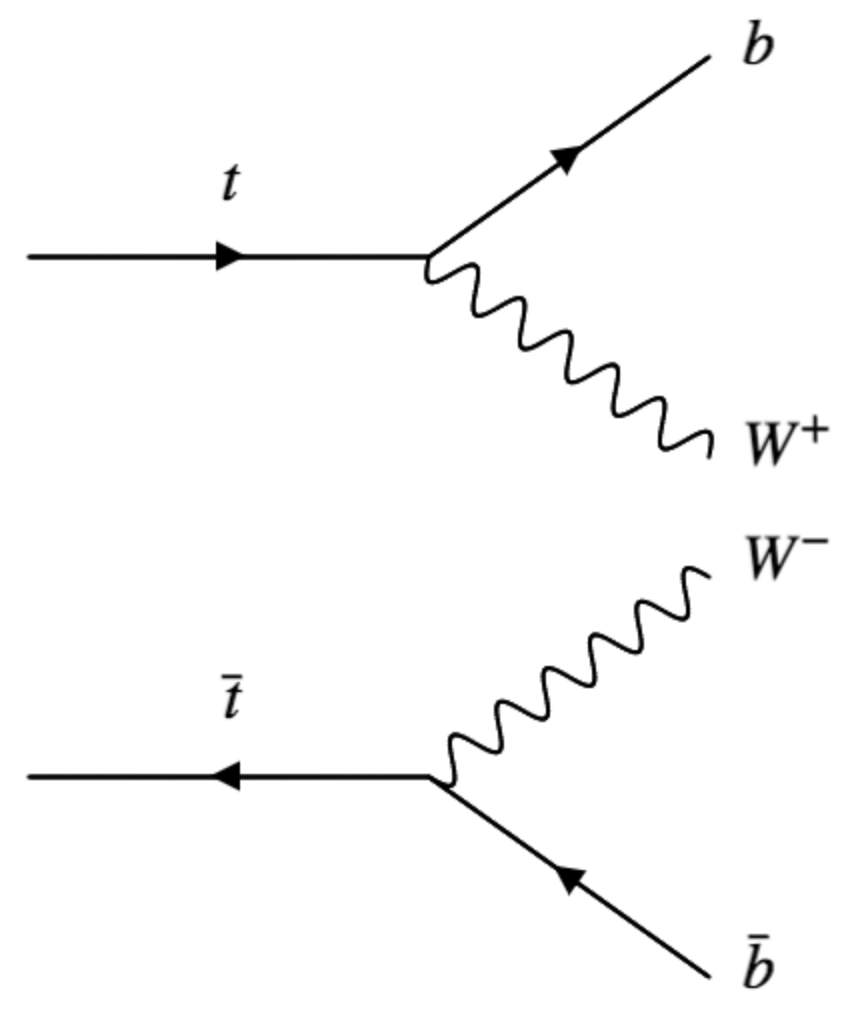
\includegraphics[width=0.4\textwidth]{Pictures/ttbar.png} a
   \caption{$t \bar{t}$ pair decaying to $b \bar{b}$ and two $W$ bosons}
   \label{fig:ttbar}
\end{figure}

\noindent In either the $t$ or the $\bar{t}$ scenarios, the resultant bottom quark, or anti-quark, will thusly initiate a hadronic jet, referred to as $b$-jets.
As described in \ref{subsec:bjetTag}, $b$-jets have very characteristic properties making them recognisable in the analysis and allowing for them to be tagged as $b$-jets
As a result of this b-jet tagging, one is able to specify whether or not to include them in the search criteria.
Seeing as we are not looking for hadronic final states from the SUSY interaction, the search criteria ignores all tagged $b$-jets signals.

\subsection{Mass Shells}
Within the overall interaction, specifically in the $\tilde{\chi}^{0}_{2}$ decay, there is the possibility of producing an on shell or an off shell $Z$ boson. 
More interpretably, this means that one either has a real or a virtual $Z$ boson.
When examining the the leptons associated with the $Z$ boson decay, one is able to construct and invariant mass.
From the on shell lepton pair one should be able to reconstruct the mass of the real $Z$ boson, however, virtual $Z$ bosons may result in the reconstruction of a mass significantly above or below the true value.
This is not an issue as it allows for a splitting in analysis procedure. 
One can thereby examine on shell and off shell events separately.

Below shows the invariant mass distribution of the two leptons associated with the $Z$ boson.

\begin{figure}[H] %  figure placement: here, top, bottom, or page
   \centering
   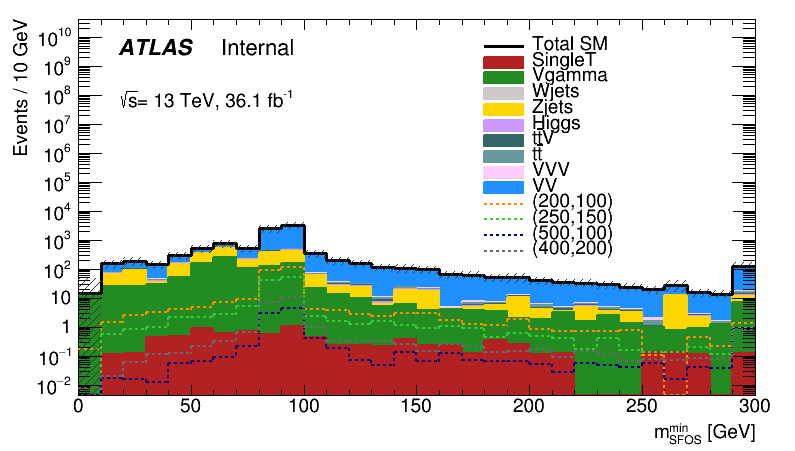
\includegraphics[width=0.7\textwidth]{Pictures/ZmassDist.png} 
   \caption{Invariant mass distribution of same flavour, opposite sign lepton pair}
   \label{fig:L1L2InvariantMass}
\end{figure}

\noindent The solid coloured blocks capped with the thick black line are the Standard Model backgrounds with the dashed lines representing the simulated SUSY grid samples.
We can see clearly that there exists a peak in the distribution of both the backgrounds and the samples centred at roughly $90$ GeV, spanning from $80 - 100$ GeV.
This is clearly a $Z$ mass peak and so we can divide analyses accordingly.
Luckily, the mass of the $Z$ boson is a well known quantity and so we are able to define mass shell regions with a high degree of specificity.
The agreed requirements for the on and off shell analyses are thereby defined as:

\begin{align} 
\textrm{On Shell:}\ \ &m_{\textrm{SFOS}}^{min} \in [81.2, 101.2] \\
\textrm{Off Shell:}\ \ &m_{\textrm{SFOS}}^{min} \notin [81.2, 101.2].
\end{align}

\begin{figure}[H]
    \centering
    \begin{subfigure}[b]{0.48\textwidth}
        \centering
        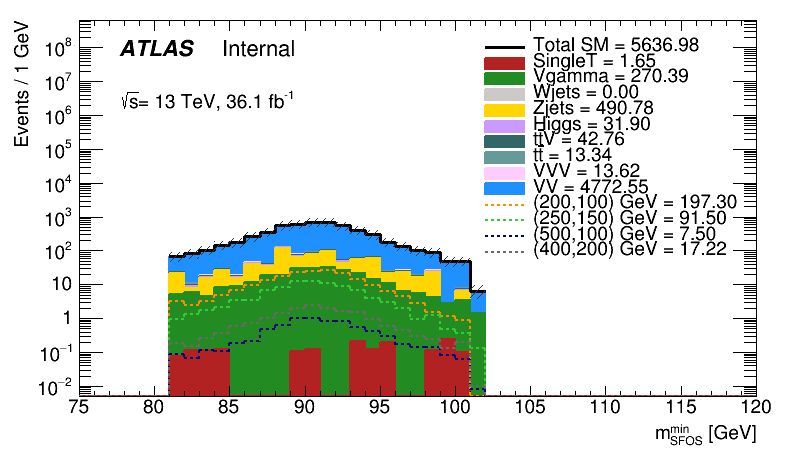
\includegraphics[width=\textwidth]{Pictures/OnMassShell.png}
    \caption{}
    \end{subfigure}
    ~
    \begin{subfigure}[b]{0.48\textwidth}
        \centering
        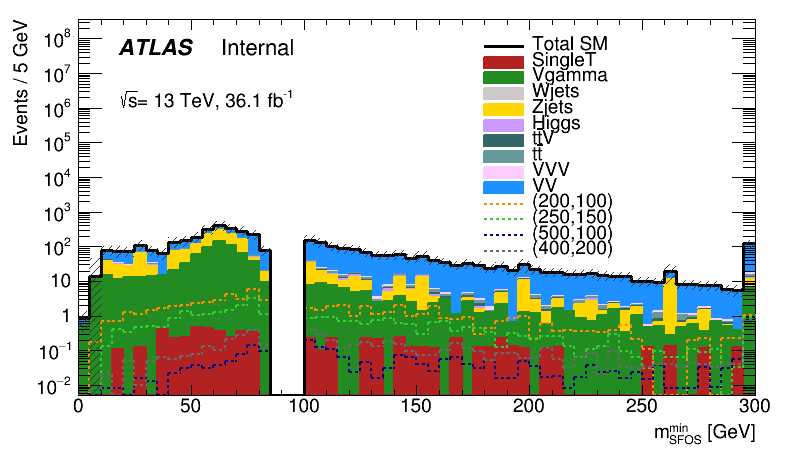
\includegraphics[width=\textwidth]{Pictures/OffMassShell.png}
    \caption{}    
        \end{subfigure}
\caption{(a) On shell invariant mass distribution of same flavour, opposite sign lepton pair.
(b) Off shell invariant mass distribution of same flavour, opposite sign lepton pair.}
\label{fig:}
\end{figure}

With these considerations in mind, the list of requirements for the signal selection are as follows.

\begin{table}[H]
\begin{center}
\begin{tabular}{l | c}
\toprule
Cut & Event Selection \\
\hline
Leptons & $\ell^{+} \ell^{-} \ell$ \\
\hline \hline
number $b$-jets & 0 \\
\hline
$m_{SFOS}^{min}$ & $\in/\notin [81.2, 101.2]$ GeV \\
\bottomrule
\end{tabular}
\end{center}
\caption{Minimum requirements for signal selection}
\label{tab:minCuts}
\end{table}

\noindent It is with these requirements that one is able to show the first extent of the background count reduction.
The selections, as given in table \ref{tab:minCuts}, was implemented within the Y{\scshape ield Table} framework.
So as to give a direct comparison, the script was asked to first produce a count when only a tri-leptonic signature was seen, then  a count when the on shell requirements were met, and finally a count when the off shell requirements were met.
The results of these cuts being applied are shown below.

\begin{table}[H]
\begin{center}
\begin{tabular}{c r r r}
\toprule
Sample& No Selection applied& on Z mass shell& off Z mass shell\\

\midrule
$t\bar{t}$V& $ 425.65 \pm 1.29 $& $ 42.76 \pm 0.46 $& $ 21.45 \pm 0.31 $\\

$t\bar{t}$& 	 $299.83\pm 4.5$& 	 $13.34\pm 0.95$& 	 $61.33\pm 2.05$\\

single $t$& 	 $18.4\pm 1.46$& 	 $1.65\pm 0.43$& 	 $6.67\pm 0.89$\\

$Z$+jets& 	 $1471.08\pm 120.23$& 	 $490.78\pm 62.66$& 	 $874.32\pm 100.85$\\

$W$+jets& 	 $0.23\pm 0.15$& 	 $0.0\pm 0.0$& 	 $0.08\pm 0.07$\\

Dibosons& 	 $7455.16\pm 17.85$& 	 $4772.79\pm 14.91$& 	 $2376.64\pm 9.51$\\


V$\gamma$& 	 $1059.41\pm 17.91$& 	 $270.39\pm 8.88$& 	 $757.5\pm 15.27$\\

Higgs& 	 $81.88\pm 4.83$& 	 $31.9\pm 3.0$& 	 $29.88\pm 3.26$\\

Tribosons& 	 $54.95\pm 0.67$& 	 $13.62\pm 0.28$& 	 $30.26\pm 0.52$\\

\hline
Total background& 	 $10866.58\pm123.05$& 	 $5637.22\pm65.1$& 	 $4158.14\pm102.52$\\

\hline\hline
via WZ (200,100)& 	 $267.35\pm 4.51$& 	 $197.3\pm 3.87$& 	 $64.29\pm 2.21$\\

via WZ (250,150)& 	 $124.57\pm 2.02$& 	 $91.5\pm 1.73$& 	 $30.31\pm 1.00$\\

via WZ (400,200)& 	 $23.88\pm 0.5$& 	 $17.22\pm 0.42$& 	 $6.12\pm 0.25$\\

via WZ (500,100)& 	 $10.79\pm 0.3$& 	 $7.5\pm 0.25$& 	 $2.9\pm 0.15$\\
\bottomrule
\end{tabular}
\end{center}
\caption{Initial yields from background and samples after applying initial selection criteria}
\label{tab:preselection}
\end{table}

The first noticeable effect of these cuts, when applied on shell, is that the events containing top quarks are reduced to around 10\% of their initial values.
Another noticeable effect is that the events recorded as a result of $W+$ jets has been reduced entirely. 
This particular background was initially negligible in comparison to the other background sources, never the less, this is still a positive result for the selection criteria.
Furthermore, Higgs and tri-boson events have both been reduced to around a third of their initial values.
This is also true for $Z+$jets and V$\gamma$, however, they are much more prominent still and so further limitations must be placed in order to reduce them to a manageable level.

The obviously dominating background is the diboson events, making up 85\% of the total recorded background yield. 
Seeing as dibosonic events exactly mimic the desired supersymmetric interaction signal, naturally one expects it to be the dominating background.
Despite this, the total number of background counts is reduced by roughly one half, offering promise for the continuation of the selection criteria

When assessing the off shell yields it is clear that there are differing levels of success in particular samples, yet overall the totals yield similar success.
The backgrounds involving top quarks are all reduced substantially, with $t\bar{t}$V being reduced to 5\% of its original value.
Comparatively to the on shell yields the other two top quark backgrounds are reduced to a much lesser extent.
This is also true for $Z+$jets, however, logically this is reasonable as with the off shell requirements one is allowing for a much larger range of values for the invariant mass of the leptons associated with the $Z$ boson.

One of the bigger differences between the on and off shell yields comes from the diboson background.
We see that when taken off shell this background is reduced to roughly 30\% of its original value.
This is good as it shows a direct way of attenuating diboson events, however, they still make up a majority of the overall background count.

When considering the sample yields the most notable effect is that the off shell condition removes much more of the signal than the on shell condition.
The general reduction in signal is of about 30\% when applying on shell requirements, where as the loss of signal when applying off shell requirements is up to 75\%.
Lastly, it appears that there are more sample events recorded that satisfy the selection criteria when the mass of the $\tilde{\chi}^{\pm}_{1}$ or $\tilde{\chi}^{0}_{2}$ is lower.
This is a feature that is considered through the duration of the analysis when applying further cuts for the selection criteria.

\section{Optimising On Shell Selection with Kinematic Variable Cuts} \label{sec:OnShellOpt}
The basic selection criteria offer substantial reduction in background event yield with compensatory loss in signal yield.
In order to develop a more complete set of selection criteria examination of kinematic variables must be conducted.
This is done not only to further reduce the background counts, but also to improve the signal significance of the samples with respect to the background.

The important variables considered in this stage of the analysis are the missing transverse energy, $E_{T}^{miss}$, and the transverse momentum of the final state leptons, $p_{T}^{\ell_{i}}$.
In order to place qualified conditions on these variables, examinations of their initial states must be made along with considerations of how the variables change when conditions are applied to other variables.

Numerous criteria are considered while placing preliminary cuts on variables, including general form of the variable and how the signal and the background relate to one another.
However, a general rule of thumb is to examine the significance traces of the sample signals with the associated variables and apply a cut in accordance with a region of increasing significance.
This is done in order to eliminate regions where the spectrum is dominated by background and, ideally, preserve regions where the signal is of increased significance. 
This method is applied both to the on shell and off shell baselines in order to achieve a more complete set of criteria for the signal selection process.  

\begin{figure}[H]
    \centering
    \begin{subfigure}[b]{0.48\textwidth}
        \centering
        \includegraphics[width=\textwidth]{Pictures/eT_miss}
    \caption{$E_{T}^{miss}$}
    \end{subfigure}
    ~
    \begin{subfigure}[b]{0.48\textwidth}
        \centering
        \includegraphics[width=\textwidth]{Pictures/LepPt[0]}
    \caption{$p_{T}^{\ell_{1}}$}    
        \end{subfigure}
    ~
    \centering
    \begin{subfigure}[b]{0.48\textwidth}
        \centering
        \includegraphics[width=\textwidth]{Pictures/LepPt[1]}
    \caption{$p_{T}^{\ell_{2}}$}
    \end{subfigure}
    ~
    \begin{subfigure}[b]{0.48\textwidth}
        \centering
        \includegraphics[width=\textwidth]{Pictures/LepPt[2]}
    \caption{$p_{T}^{\ell_{3}}$}    
        \end{subfigure}
\caption{Initial plot of kinematic variables with on shell selection criteria applied}
\label{fig:initialKinematics}
\end{figure}

\subsection{Preliminary cut on $E_{T}^{miss}$}
In figure \ref{fig:initialKinematics}a we see a higher propensity to lower values of $E_{T}^{miss}$ in the background signal, as well as the two light weight SUSY samples.
Starting at about 60 GeV the background along with the two sample signals all gradually decrease while going towards higher energy.
This is not true for the higher mass samples which gradually increase over the spectrum until meeting the other sample signals at about 220 GeV.
The significance (Zn) traces, however, indicate that at about 60 GeV the signals and background become more closely spaced, as shown in the increase of Zn most dramatically in the (200,100) sample.
For this reason a preliminary cut is placed at 60 GeV on the missing transverse energy, excluding the events with energy below that.

\begin{figure}[H] %  figure placement: here, top, bottom, or page
   \centering
   \includegraphics[width=0.5\textwidth]{Pictures/eT_miss_withArrow} 
   \caption{Preliminary cut on $E_{T}^{miss}$ for the on shell analysis before variable optimisation}
   \label{fig:example}
\end{figure}

\subsection{Preliminary cut on $p_{T}^{\ell_{1}}$}

Placing the preliminary cuts on the lepton transverse momenta follow the same general process as described for the missing transverse energy.
In figure \ref{fig:initialKinematics}b we notice that the lower mass samples follow the same general form as the background level, however, the signals and the background become more closely interspaced at approximately 40 GeV, as shown by the increase in the Zn curve at the same energy value.
It is also obvious that the heavier sample signals only begin at 35 GeV and slowly rise until eventually reaching the same general signal level as the lighter samples.
This is, however, only at much higher energy.

This light sample signal significance increase, along with the start of the heavier sample signals all at the same value gives an indication that one may initially place the cut at 40 GeV, excluding all events with lower energy values.
Fortunately, this removes a good portion of the background spectrum, however, a non negligible portion of the low mass samples is also omitted. 
This is not as detrimental for the heavier samples as barely any of the sample signal is removed by this cut. 

\begin{figure}[H] %  figure placement: here, top, bottom, or page
   \centering
   \includegraphics[width=0.5\textwidth]{Pictures/LepPt[0]_withArrow} 
   \caption{Preliminary cut on $p_{T}^{\ell_{1}}$ for the on shell analysis before variable optimisation}
   \label{fig:example}
\end{figure}

\subsection{Preliminary cut on $p_{T}^{\ell_{2}}$}

When considering figure \ref{fig:initialKinematics}c we notice that the peak is much more compressed towards the lower values, as opposed to the broader peak in the distribution of the transverse momentum of the leading lepton.
Taking into consideration the significance curves one notices that there is a distinct increase in all of the traces at 30 GeV.
As a preliminary, exclusion of events below 30 GeV would remove vastly more background events than one stands to lose in sample signal.
It was decided thereof that the initial cut would be placed there in order to initiate the optimisation further into the analysis.

\begin{figure}[H] %  figure placement: here, top, bottom, or page
   \centering
   \includegraphics[width=0.5\textwidth]{Pictures/LepPt[1]_arrow} 
   \caption{Preliminary cut on $p_{T}^{\ell_{2}}$ for the on shell analysis before variable optimisation}
   \label{fig:example}
\end{figure}

\subsection{Preliminary cut on $p_{T}^{\ell_{3}}$}

Figure \ref{fig:initialKinematics}d shows a monotonically decreasing spectrum in both the backgrounds and the sample signals.
In this spectrum, however, the lightest sample - given by the orange line - remains quite close to the overall background signal.
Upon consideration of the significance lines one can see in all of the trances, however most prominently in the orange line, that there is a clear increase at 25 GeV.
The preliminary cut is thereby places at 25 GeV, removing a non-negligible amount of background signal, with the slight trade off of losing a portion of each of the sample signals.

\begin{figure}[H] %  figure placement: here, top, bottom, or page
   \centering
   \includegraphics[width=0.5\textwidth]{Pictures/LepPt[2]_arrow} 
   \caption{Preliminary cut on $p_{T}^{\ell_{3}}$ for the on shell analysis before variable optimisation}
   \label{fig:example}
\end{figure}

\subsection{Optimisation of the on shell preliminary cuts}
In order to optimise the position of the cuts made on the kinematic variables, one must consider how each cut affects the other variables as all of the kinematics of the system are inherently connected.
The approach used in this analysis is, for each variable, to examine the spectra will all but one of the previously described preliminary cuts applied and then consider if the position of these preliminary cuts can be made better or should be kept constant.
These "all but one" plots are referred to as "N-1" plots, following the common mathematical convention that the $n^{th}$ value is the last.

Considering first the missing transverse energy, plots were made excluding $p_{T}^{\ell_{1}}$, $p_{T}^{\ell_{2}}$, and $p_{T}^{\ell_{3}}$ individually.
The full collection of N-1 plots for $E_{T}^{miss}$, on shell, can be found in Appendix \ref{app:n-1onZ}, figures \ref{fig:METN-1ON}a, b, and c.

\begin{figure}[H] %  figure placement: here, top, bottom, or page
   \centering
   \includegraphics[width=0.6\textwidth]{Pictures/eT_miss_noLepPt[0].png} 
   \caption{$E_{T}^{miss}$ with $p_{T}^{\ell_{2}}$ and $p_{T}^{\ell_{3}}$ cuts but not $p_{T}^{\ell_{1}}$ cut}
   \label{fig:METONN-1LepPt[0]}
\end{figure}

Figure \ref{fig:METONN-1LepPt[0]} shows the $E_{T}^{miss}$ spectrum with forward cuts applied at 30 GeV on $p_{T}^{\ell_{2}}$ and 25 GeV on $p_{T}^{\ell_{3}}$. 
Noticeably from this plot one can see that the point at which the significance trace of the (200,100) sample crosses the zero line has been moved to a lower energy value, this time at 50 GeV.
Correspondingly, the significance traces of the other samples also show an increase in gradient at roughly 50 GeV.
This is true also for the N-1 plots that exclude the other lepton transverse momenta, giving motivation for the $E_{T}^{miss}$ cut to be relaxed to 50 GeV.
This is beneficial as excluding events with energy below 50 GeV eliminates the peak of the background spectrum whilst retaining a good portion of the sample signals.

\begin{figure}[H] %  figure placement: here, top, bottom, or page
   \centering
   \includegraphics[width=0.6\textwidth]{Pictures/LepPt[0]_noeT_miss} 
   \caption{$p_{T}^{\ell_{1}}$ with $p_{T}^{\ell_{2}}$ and $p_{T}^{\ell_{3}}$ cuts but not $E_{T}^{miss}$ cut}
   \label{fig:LepPt[0]ONN-1MET}
\end{figure}

Figure \ref{fig:LepPt[0]ONN-1MET} we see the the momentum spectrum of the leading lepton with the $p_{T}^{\ell_{2}}$ and $p_{T}^{\ell_{3}}$ cuts applied at 30 GeV and 25 GeV respectively.
Upon consideration of this plot and those shown in figures figures \ref{fig:LepPt[0]N-1ON}a, b, and c, is can be seen that the significance traces show the most noticeable change in gradient at approximately 50 GeV. 
A cut at 50 GeV would exclude a large portion of the background spectrum in the region where the total level is rising before the peak in the spectrum.
By comparison, very little of the high mass sample signals are lost, however, a non-negligible amount of the low mass samples are omitted.   
This can still be considered a worth while cut as the signal significance for low energy do not show that the region is particularly interesting.

\begin{figure}[H] %  figure placement: here, top, bottom, or page
   \centering
   \includegraphics[width=0.6\textwidth]{Pictures/LepPt[1]_noLepPt[0]} 
   \caption{$p_{T}^{\ell_{2}}$ with $E_{T}^{miss}$ and $p_{T}^{\ell_{3}}$ cuts but not cut  $p_{T}^{\ell_{1}}$}
   \label{fig:LepPt[1]ONN-1MET}
\end{figure}

\noindent Figure \ref{fig:LepPt[1]ONN-1MET}, above, shows the transverse momentum spectrum of the next to leading lepton with all but the $p_{T}^{\ell_{1}}$ cut applied.
In consideration of this and the other plots in figure \ref{fig:LepPt[1]N-1ON} it was decided that the cut on this variable should be made in accordance with the hard cut from the signal generation, shown to be 25 GeV.
Obviously this includes the entire spectrum in the event selection, however, with consideration of the yields shown in the legend of the plot the amount of background is still dramatically reduced, and the sample yields are kept at a reasonable high level.

\begin{figure}[H] %  figure placement: here, top, bottom, or page
   \centering
   \includegraphics[width=0.6\textwidth]{Pictures/LepPt[2]_noLepPt[1]} 
   \caption{$p_{T}^{\ell_{3}}$ with $E_{T}^{miss}$ and $p_{T}^{\ell_{1}}$ cuts but not cut  $p_{T}^{\ell_{2}}$}
   \label{fig:LepPt[2]ONN-1LepPt[1]}
\end{figure}

\noindent In the $p_{T}^{\ell_{3}}$ spectrum, above, all cuts except for the cut on $p_{T}^{\ell_{2}}$.
The general form of the spectrum follows the same trend as seen before for this variable. 
With this spectrum, and the spectra shown in figure \ref{fig:LepPt[2]N-1ON}, it is clear that the cut being placed at 25 GeV appears to the the optimum location.
This is shown by the increase in the significance traces of all of the samples at 25 GeV.

\subsection{Results of the on shell optimisation}
With all of the considerations as described above one is able to write down the full list of signal selection criteria for the on mass shell portion of the analysis.

\begin{table}[H]
\begin{center}
\begin{tabular}{l | c}
\toprule
Cut & Event Selection \\
\hline
Leptons & $\ell^{+} \ell^{-} \ell$ \\
\hline \hline
number $b$-jets & 0 \\
\hline
$m_{SFOS}^{min}$ & $\in [81.2, 101.2]$ GeV \\
\hline
$p_{T}^{\ell_{1}}$ & $>$50 GeV \\
\hline
$p_{T}^{\ell_{2}}$ & $>$25 GeV \\
\hline
$p_{T}^{\ell_{3}}$ & $>$25 GeV \\
\hline
$E_{T}^{miss}$ & $>$50 GeV \\
\bottomrule
\end{tabular}
\end{center}
\caption{table of event selection cuts for the on $Z$ mass shell analysis}
\label{tab:onShellConditions}
\end{table}

\noindent With all of these selection criteria applied and implemented within the Y{\scshape field Table} framework a table of event yields for each of the background sources and sample signals can be calculated.
The result of this implementation is as follows.

\begin{table}[H]
\begin{center}
\begin{tabular}{c r r r r r r r}
\toprule
Sample& on shell with preselection & on shell with full selection\\

\midrule
$t\bar{t}$V&  $ 42.76 \pm 0.46 $& $ 22.35 \pm 0.32 $\\

$t\bar{t}$&  	 $13.34\pm 0.95$& 	 $3.36\pm 0.48$\\

single $t$&  	 $1.65\pm 0.43$& 	 $0.25\pm 0.17$\\

$Z$+jets& 	 $490.78\pm 62.66$& 	$45.62\pm 8.79$\\

$W$+jets&  	 $0.0\pm 0.0$& 	 $0.0\pm 0.0$\\

Dibosons&  	 $4772.79\pm 14.91$& 	 $1415.71\pm 8.09$\\

V$\gamma$&  	 $270.39\pm 8.88$& 	 $7.99\pm 1.36$\\

Higgs& 	 $31.9\pm 3.0$& 	 $9.39\pm 1.64$\\

Tribosons&  	 $13.62\pm 0.28$& 	 $7.02\pm 0.2$\\

\hline
Total background&  	 $5637.22\pm65.10$& 	 $1511.68\pm12.16$\\

\hline\hline
via WZ (200,100)&  	 $197.3\pm 3.87$& 	 $96.42\pm 2.74$\\

via WZ (250,150)&  	 $91.5\pm 1.73$& 	 $45.33\pm 1.23$\\

via WZ (400,200)& 	 $17.22\pm 0.42$& 	 $13.72\pm 0.38$\\

via WZ (500,100)&	 $7.5\pm 0.25$& 	 $6.85\pm 0.24$\\

\bottomrule
\end{tabular}
\end{center}
\caption{signal and background yields after applying all selection cuts for on shell analysis}
\label{tab:onshellResults}
\end{table}

We see from table \ref{tab:onshellResults} that with the full compliment of cut and conditions stated in table \ref{tab:onShellConditions}, for most of the background sources the yields have been dramatically.
Single $t$ and $t\bar{t}$ have both been reduced by an order magnitude, with single $t$ having less than one event recorded during the entire selection process.
$Z+$jets and V$\gamma$ backgrounds which previously were two of the highest contributing background events have been substantially reduced, with V$\gamma$ becoming one of the more infrequently recorded events. 

Catalogued diboson events have undergone a reduction of approximately 70\% showing great motivation for the validity of the selection cuts.
Despite this dramatic reduction diboson events continue to dominate the overall background, dwarfing the total sample signal yields.
From this result it is clear that further conditions must be added to the selection criteria in order to reduce background levels further. 

The sample signal yields show an interesting effect as a result of the selection criteria.
For the lower mass samples, the yields between preselection and full selection have halved. 
Interestingly, however, the higher mass samples show far less reduction in signal yield, with the (400,200) being reduced by 20\% and the (500,100) sample being reduced by 8\%.
This is affirmation of the observations made in the variable plots showing that the sample signals start at much higher energies as compared to the lower mass samples.
An interesting extension of the analysis could then be to treat higher mass and lower mass samples with different selection criteria so as to optimise signal significance as accurately.

\section{Optimising Off Shell Selection with Kinematic Variable Cuts}
The optimisation of the off shell selection criteria is conducted similarly to that described in \ref{sec:OnShellOpt}.
That process being: apply initial selection criteria, examen the spectra of the kinematic variables in question, apply cuts on these variables, and optimise these cuts by examining the "N-1" plots. 
The results of the off shell optimisation do not necessarily have to be the same as the on shell optimisation as differing initial selection criteria may alter the kinematics further into the selection process.

\begin{figure}[H]
    \centering
    \begin{subfigure}[b]{0.48\textwidth}
        \centering
        \includegraphics[width=\textwidth]{Pictures/eT_miss_off}
    \caption{$E_{T}^{miss}$}
    \end{subfigure}
    ~
    \begin{subfigure}[b]{0.48\textwidth}
        \centering
        \includegraphics[width=\textwidth]{Pictures/LepPt[0]_off}
    \caption{$p_{T}^{\ell_{1}}$}    
        \end{subfigure}
    ~
    \centering
    \begin{subfigure}[b]{0.48\textwidth}
        \centering
        \includegraphics[width=\textwidth]{Pictures/LepPt[1]_off}
    \caption{$p_{T}^{\ell_{2}}$}
    \end{subfigure}
    ~
    \begin{subfigure}[b]{0.48\textwidth}
        \centering
        \includegraphics[width=\textwidth]{Pictures/LepPt[2]_off}
    \caption{$p_{T}^{\ell_{3}}$}    
        \end{subfigure}
\caption{Initial plot of kinematic variables with off shell selection criteria applied}
\label{fig:initialKinematicsOff}
\end{figure}

\subsection{Preliminary Cut on $E_{T}^{miss}$}
In figure \ref{fig:initialKinematicsOff}a we see that the majority of the background is concentrated into the lower energy region of the $E_{T}^{miss}$ spectrum. 
This is also true for the low mass sample signals, however, the higher mass samples show a steady increase as energies missing transverse energy gets larger.
It is immediately clear that if a cut is placed that excludes the lower portion of the spectrum, a significant number of background events can be removed.

Upon consideration of the significance traces, it is clear that the lower mass samples show more rapid increase, as is expected from the shape of their traces in the main spectrum.
The higher mass samples show a slower increase that the low mass samples, with a good point of increasing gradient at approximately 60 GeV.
This value is chosen as although one loses a significant portion of the low mass signal one excludes the region of the spectrum that is overwhelmed by the background signal

\begin{figure}[H] %  figure placement: here, top, bottom, or page
   \centering
   \includegraphics[width=0.6\textwidth]{Pictures/eT_miss_withArrow_off} 
   \caption{Preliminary cut on $E_{T}^{miss}$ for the off shell analysis before optimisation}
   \label{fig:example}
\end{figure}

\subsection{Preliminary Cut on $p_{T}^{\ell_{1}}$}
In figure \ref{fig:initialKinematicsOff}b we see a very steep rise in the background signal, reaching a peak value at approximately 35 GeV.
The total background then gradually decreases over the rest of the spectrum.
Looking at the sample traces, we see that the lower mass samples start at 25 GeV as opposed to the 20 GeV for the background signal.
The higher mass sample signals start at higher energy still, a feature previously noticed in many other spectra. 

Due to the very steep rise in the background compared to the more gradual rise in the sample signals, there is a large disparity between signal and background at low energy.
This is shown in the significance traces as it is only at approximately 40 GeV that we see a rise in the sample signals, the weakest of which come, again, from the higher mass samples.
For this reason the preliminary cut on this variable is placed at 40 GeV.

\begin{figure}[H] %  figure placement: here, top, bottom, or page
   \centering
   \includegraphics[width=0.6\textwidth]{Pictures/LepPt[0]_withArrow_off} 
   \caption{Preliminary cut on $p_{T}^{\ell_{1}}$ for the off shell analysis before optimisation}
   \label{fig:example}
\end{figure}

\subsection{Preliminary Cut on $p_{T}^{\ell_{2}}$}

In figure \ref{fig:initialKinematicsOff}c we see that the peak of the distribution is very early in the spectrum, roughly at 25 GeV.
The background is, essentially, constantly decreasing over the range of the spectrum, whereas the sample signals show an initial increase in amplitude leading to a gradual decline as the spectrum goes to higher energies.
Looking at the significance traces one notices that there is a common increase in gradient at 30 GeV.
This increase is attributed to the sample signals and the background becoming more closely interspaced due to the aforementioned differences in their profiles.
It is for this reason that the initial cut for $p_{T}^{\ell_{2}}$ is placed at 30 GeV.

\begin{figure}[H] %  figure placement: here, top, bottom, or page
   \centering
   \includegraphics[width=0.6\textwidth]{Pictures/LepPt[1]_withArrow_off} 
   \caption{Preliminary cut on $p_{T}^{\ell_{2}}$ for the off shell analysis before optimisation}
   \label{fig:example}
\end{figure}

\subsection{Preliminary Cut on $p_{T}^{\ell_{3}}$}

Lastly, figure \ref{fig:initialKinematicsOff}d shows the spectrum of the transverse momentum of the lepton associated with the $W$ boson.
In this spectrum we see that the background is monotonically decreasing in the range 20 GeV to 170 GeV.
This is true for the sample signals too, however, as the samples show a different profile to their shapes we see some variations in the significance.
At approximately 25 GeV we see a slight increase in the gradient of the low mass sample significance traces, with the higher mass samples increasing far more subtly.
As a preliminary an exclusion of events with $p_{T}^{\ell_{3}}$ lower than 25 GeV is applied.

\begin{figure}[H] %  figure placement: here, top, bottom, or page
   \centering
   \includegraphics[width=0.6\textwidth]{Pictures/LepPt[2]_withArrow_off} 
   \caption{Preliminary cut on $p_{T}^{\ell_{3}}$ for the off shell analysis before optimisation}
   \label{fig:example}
\end{figure}

\subsection{Optimisation of the off shell preliminary cuts}
The optimisation of the off shell selection criteria is carried out in the same way as described for the on shell analysis.
Plots of variables with all but one of the preliminary cuts applied are made, assessed, and alterations are made if required.


\begin{figure}[H]
    \centering
    \begin{subfigure}[b]{0.48\textwidth}
        \centering
        \includegraphics[width=\textwidth]{Pictures/eT_miss_noLepPt[0]_off}
    \caption{}
    \end{subfigure}
    ~
    \begin{subfigure}[b]{0.48\textwidth}
        \centering
        \includegraphics[width=\textwidth]{Pictures/eT_miss_noLepPt[1]_off}
    \caption{}    
        \end{subfigure}
\caption{$E_{T}^{miss}$ with $p_{T}^{\ell_{2}}$ and $p_{T}^{\ell_{3}}$ cuts but not $p_{T}^{\ell_{1}}$ cut (left) and $E_{T}^{miss}$ with $p_{T}^{\ell_{1}}$ and $p_{T}^{\ell_{2}}$ cuts but not $p_{T}^{\ell_{2}}$ cut (right)}
\label{fig:METN-1OFF}
\end{figure}

Figure \ref{fig:METN-1OFF} show the N-1 plots for $E_{T}^{miss}$ excluding different transverse momenta in each spectrum.
No major difference in the shape of the background and signal is noticeable.
It was decided that the cut on missing transverse energy should remain at 60 GeV, excluding all events with lower energy.
This is in accordance with each the significances' gradients increasing at this point.  
Exclusion of the lower energy events takes away a substantial number of the background events as there is a large clustering of low energy background.
A large portion of the low mass sample signals will be lost, however, the higher mass sample signals comparatively lose very little. 

\begin{figure}[H] %  figure placement: here, top, bottom, or page
   \centering
   \includegraphics[width=0.6\textwidth]{Pictures/LepPt[0]_noMET_off} 
   \caption{$p_{T}^{\ell_{1}}$ with $p_{T}^{\ell_{2}}$ and $p_{T}^{\ell_{3}}$ cuts but not $E_{T}^{miss}$ cut}
   \label{fig:LepPt[0]N-1MET}
\end{figure}

In figure \ref{fig:LepPt[0]N-1MET}, we see the transverse momentum spectrum of the leading lepton with the cuts to the second and third lepton, but excluding the cut on missing transverse energy.
It is noticeable that the rise in the low energy region of the spectrum has become more abrupt, however, a significant about of the background level has been removed. 
The significance traces show the same trend as before: a small but noticeable rise at approximately 40 GeV.
From this we can infer that the preliminary cut on $p_{T}^{\ell_{1}}$ was in the optimum place, and so the cut is left where it is. 

\begin{figure}[H] %  figure placement: here, top, bottom, or page
   \centering
   \includegraphics[width=0.6\textwidth]{Pictures/LepPt[1]_noeT_missoff} 
   \caption{$p_{T}^{\ell_{2}}$ with $p_{T}^{\ell_{1}}$ and $p_{T}^{\ell_{3}}$ cuts but not $E_{T}^{miss}$ cut}
   \label{fig:LepPt[1]N-1MET}
\end{figure}

Figure \ref{fig:LepPt[1]N-1MET} shows the transverse momentum spectrum of the next to leading lepton with cuts applied to the first and third leptons' momenta, and excluding the cut on missing transverse energy.
In its form, this spectrum looks similar to how it did without the additional cuts applied.
The significance traces of the sample signals, however, do not align with one another in terms of an increase in gradient.
Seeing this is quite a weak variable in terms of its effect on the distributions of other variables, it was decided that the cut should be applied in accordance with the hard cut from the event generation; that is at 25 GeV, as set by the event generating Monte Carlo.

\begin{figure}[H] %  figure placement: here, top, bottom, or page
   \centering
   \includegraphics[width=0.6\textwidth]{Pictures/LepPt[2]_noeT_miss_off} 
   \caption{$p_{T}^{\ell_{3}}$ with $p_{T}^{\ell_{1}}$ and $p_{T}^{\ell_{2}}$ cuts but not $E_{T}^{miss}$ cut}
   \label{fig:LepPt[2]N-1MET}
\end{figure}

Figure \ref{fig:LepPt[2]N-1MET} shows the effects of the cuts as they are applied to the transverse momentum of the lepton associated with the $W$ boson.
In this spectrum we see that there is a subtle increase in significance of the low mass samples, positioned at approximately 25 GeV.
Despite this, very little can be seen in the other N-1 plots of this variable and so this does not give enough evidence to place a definitive cut at 25 GeV.
In accordance with the hard cut defined by the Monte Carlo event generation, the cut on $p_{T}^{\ell_{3}}$ was made at 20 GeV. 

\subsection{Results of the off shell optimisation}
With all of the evidence described above, the list of selection criteria and kinematic cuts for the off shell analysis is as follows.

\begin{table}[H]
\begin{center}
\begin{tabular}{l | c}
\toprule
Cut & Event Selection \\
\hline
Leptons & $\ell^{+} \ell^{-} \ell$ \\
\hline \hline
number $b$-jets & 0 \\
\hline
$m_{SFOS}^{min}$ & $\notin [81.2, 101.2]$ GeV \\
\hline
$p_{T}^{\ell_{1}}$ & $>$40 GeV \\
\hline
$p_{T}^{\ell_{2}}$ & $>$25 GeV \\
\hline
$p_{T}^{\ell_{3}}$ & $>$20 GeV \\
\hline
$E_{T}^{miss}$ & $>$60 GeV \\
\bottomrule
\end{tabular}
\end{center}
\caption{table of event selection cuts for the off $Z$ mass shell analysis}
\label{tab:offShellConditions}
\end{table}

\noindent These conditions are thusly implemented within the Y {\scshape ieldTable} analysis framework, producing the event yields of all of the backgrounds and samples under the specifications of the selection criteria. 
The results are as follows.

\begin{table}[H]
\begin{center}
\begin{tabular}{c r r r r r r r}
\toprule
Sample& off shell with preselection& off shell with full selection\\

\midrule
$t\bar{t}$V& $ 21.45 \pm 0.31 $& $ 10.45 \pm 0.21 $\\

$t\bar{t}$& 	 $61.33\pm 2.05$& 	 $19.25\pm 1.15$\\

single top& 	 $6.67\pm 0.89$& 	 $1.88\pm 0.47$\\

$Z$+jets Sherpa& 	 $874.32\pm 100.85$& 	 $12.97\pm 3.74$\\

$W$+jets& 	 $0.08\pm 0.07$& 	 $0.01\pm 0.01$\\

Dibosons& 	 $2376.64\pm 9.51$& 	 $446.67\pm 4.12$\\

V$\gamma$& 	 $757.5\pm 15.27$& 	 $7.64\pm 1.45$\\

Higgs& 	 $29.88\pm 3.26$& 	 $8.22\pm 1.71$\\

Tribosons& 	 $30.26\pm 0.52$& 	 $14.25\pm 0.36$\\

\hline
Total background& 	 $4158.14\pm102.52$& 	 $521.35\pm6.14$\\

\hline\hline
via WZ (200,100)& 	 $64.29\pm 2.21$& 	 $25.17\pm 1.41$\\

via WZ (250,150)& 	 $30.31\pm 1.0$& 	 $13.24\pm 0.67$\\

via WZ (400,200)& 	 $6.12\pm 0.25$& 	 $5.19\pm 0.23$\\

via WZ (500,100)& 	 $2.9\pm 0.15$& 	 $2.77\pm 0.15$\\

\bottomrule
\end{tabular}
\end{center}
\caption{Signal and background yields after applying all selection cuts for off shell analysis}
\label{tab:offShellResults}
\end{table}

We see in table \ref{tab:offShellResults} that under the application of the off shell selection criteria, background event yields decrease substantially.
Events involving top quarks have each been reduced to around a third of their initial values.
In comparison to the on shell yields, $t\bar{t}$V is more effectively reduced, however, the $t\bar{t}$ yield for the off shell analysis is much larger than that of the on shell.

$Z+$jets and V$\gamma$ are both substantially reduced, going from two of the more prominent background signals to two distinctly average sources of background.
In comparison with on shell yields one can see that off shell the requirements remove, by proportion, far more of these background events.
Off shell $Z+$jets and V$\gamma$ undergo a reduction of 98\% and 99\% respectively, where as the on shell variables under go a reduction of 90\% and 97\% respectively.

Diboson events undergo a reduction of approximately 80\%, a significant reduction and proportionally a larger reduction than that of the on shell yield.
As before, however, diboson events continue to make up the majority of the background signal, with the yield being over twenty times that of the next most contributing background.

The sample yields show a similar effect to that seen in the on shell yields.
The lower mass samples undergo a far greater reduction in yield compared to that of the heavier samples.
This further motivates the idea of splitting the analysis from a fully inclusive list of cuts, to a collection of selection cuts and criteria that specifically target low mass and high mass samples separately. 
